
% CLEAR-MoE++ Project Report
% Compile with: pdflatex clear_moe_project_report.tex  (run twice for TOC)

\documentclass[12pt,a4paper]{article}

% ── Packages ──────────────────────────────────────────────────────────────────
\usepackage[a4paper, margin=2.5cm]{geometry}
\usepackage{graphicx}
\usepackage{amsmath,amssymb,amsfonts}
\usepackage{booktabs}
\usepackage{array}
\usepackage{multirow}
\usepackage{xcolor}
\usepackage{hyperref}
\usepackage{listings}
\usepackage{caption}
\usepackage{subcaption}
\usepackage{float}
\usepackage{fancyhdr}
\usepackage{setspace}
\usepackage{pgfplots}
\usepackage{tikz}
\usetikzlibrary{shapes.geometric, arrows.meta, positioning, backgrounds, calc}
\pgfplotsset{compat=1.18}
\usepackage{algorithm}
\usepackage{algpseudocode}
\usepackage{tabularx}
\usepackage{longtable}
\usepackage{enumitem}
\usepackage{microtype}
\usepackage{parskip}

% ── Listings style ────────────────────────────────────────────────────────────
\definecolor{codegray}{rgb}{0.95,0.95,0.95}
\definecolor{codecomment}{rgb}{0.4,0.4,0.4}
\definecolor{codestring}{rgb}{0.2,0.4,0.1}
\definecolor{codekeyword}{rgb}{0.1,0.1,0.7}

\lstdefinestyle{pythonstyle}{
  backgroundcolor=\color{codegray},
  commentstyle=\color{codecomment}\itshape,
  keywordstyle=\color{codekeyword}\bfseries,
  stringstyle=\color{codestring},
  basicstyle=\ttfamily\footnotesize,
  breaklines=true,
  captionpos=b,
  frame=single,
  framerule=0.5pt,
  rulecolor=\color{gray!50},
  language=Python,
  showspaces=false,
  showstringspaces=false,
  tabsize=4,
  numbers=left,
  numberstyle=\tiny\color{gray},
  numbersep=6pt,
  xleftmargin=14pt,
}
\lstset{style=pythonstyle}

% ── Page style ────────────────────────────────────────────────────────────────
\pagestyle{fancy}
\fancyhf{}
\fancyhead[L]{\small CLEAR-MoE++: Project Report}
\fancyhead[R]{\small Md.\ Irtiza Hossain}
\fancyfoot[C]{\thepage}
\setlength{\headheight}{14pt}

\hypersetup{
  colorlinks=true,
  linkcolor=blue!70!black,
  citecolor=green!50!black,
  urlcolor=blue!70!black,
}

% ── Macros ────────────────────────────────────────────────────────────────────
\newcommand{\clearmoep}{\textbf{CLEAR-MoE++}}
\newcommand{\eg}{\emph{e.g.}}
\newcommand{\ie}{\emph{i.e.}}
\newcommand{\etal}{\emph{et al.}}

% ══════════════════════════════════════════════════════════════════════════════
\begin{document}

% ── Cover page ────────────────────────────────────────────────────────────────
\begin{titlepage}
\centering
\vspace*{2cm}

{\LARGE\bfseries CLEAR-MoE++\par}
\vspace{0.5em}
{\Large Calibration-Driven Layer-Selective Expert Extraction\\
from Pretrained Dense Vision Backbones\\[0.3em]
with Parallelism-Aware Routing and Runtime Co-Design\par}

\vspace{2em}
{\large\textbf{Project Report: EDA and Prototype}\par}

\vspace{3em}
\hrule height 0.5pt
\vspace{1em}

\begin{tabular}{rl}
\textbf{Author:}     & Md.\ Irtiza Hossain \\
\textbf{Student ID:} & 20101481 \\
\textbf{Email:}      & md.irtiza.hossain@g.bracu.ac.bd \\
\textbf{Date:}       & May 2026 \\
\end{tabular}

\vspace{1em}
\hrule height 0.5pt
\vspace{3em}

{\large\textbf{Abstract}\par}
\vspace{0.8em}
\begin{minipage}{0.88\textwidth}
\setstretch{1.3}
Vision transformers (ViTs) execute their feed-forward network (FFN)
sub-layers uniformly for every input token, consuming approximately
two-thirds of inference floating-point operations (FLOPs) regardless
of semantic token content.
\clearmoep{} is a post-training expert extraction pipeline that
converts a pretrained dense backbone into a conditional parallel backbone
without retraining.
The pipeline scores FFN layers by activation multimodality and output
sensitivity, decomposes only the highest-scoring late-stage blocks into a
shared low-rank basis plus cluster-specific residual experts via truncated
Singular Value Decomposition (SVD) and $k$-means clustering, fits
lightweight routers, and deploys inference via seven router variants and
six dispatch backends.
This report describes the Exploratory Data Analysis (EDA) conducted
on the Imagenette dataset and the prototype pipeline built on
DeiT-Small and SegFormer-B0.
Preliminary results show that Soft-MoE and Elastic-MoE variants preserve
100\% of dense baseline accuracy, and the cuBLAS batched-GEMM dispatch
backend achieves $23.26\times$ throughput over CPU serial execution.
A roofline analysis quantifies that routers are memory-bound while expert
GEMMs remain compute-bound, identifying dispatch optimisation as the
primary engineering target.
\end{minipage}

\vfill
{\small\textit{Keywords:} mixture of experts, vision transformer, post-training extraction, conditional compute, sparse inference, semantic segmentation, dispatch strategies, roofline analysis}
\end{titlepage}

% ── Table of contents ─────────────────────────────────────────────────────────
\tableofcontents
\newpage

\setstretch{1.25}

% ══════════════════════════════════════════════════════════════════════════════
\section{Introduction and Motivation}
\label{sec:intro}

Vision transformers \cite{dosovitskiy2021vit, liu2021swin} have become the standard backbone for image classification, object detection, and semantic segmentation. Despite their accuracy, dense ViTs execute all model parameters for every input token uniformly. Background pixels, texture patches, and foreground objects carry vastly different information yet consume identical compute—a fundamental inefficiency.

Sparse Mixture-of-Experts (MoE) architectures \cite{shazeer2017outrageously} route each token to a subset of specialised sub-networks, reducing active FLOPs without proportionally reducing accuracy. However, dominant vision MoE approaches (\eg, V-MoE \cite{riquelme2021vmoe}, AdaMV-MoE \cite{chen2023adamvmoe}) require expensive from-scratch pretraining. For practitioners holding pretrained dense checkpoints, full MoE retraining is impractical.

Post-training expert extraction offers a practical alternative. MoEfication \cite{zhang2022moefication} showed that dense FFN neurons can be grouped into experts via activation clustering without any gradient computation. D2DMoE \cite{d2dmoe2024} extended this with dynamic-$k$ routing, achieving up to 30\% latency reduction on ViT-B. Berisha \etal\ \cite{berisha2025cvpr} recovered 98\% of dense accuracy with 36.3\% MAC reduction for DeiT-B.

\clearmoep{} addresses three open gaps in this literature:

\begin{enumerate}
\item \textbf{Layer selectivity.} Prior extraction methods expertise all or fixed fractions of FFN layers. AdaMV-MoE shows empirically that later transformer layers are better candidates for expertisation \cite{chen2023adamvmoe}. CLEAR-MoE++ selects layers using a composite activation-multimodality score.

\item \textbf{Shared structure.} Disjoint expert extraction discards common visual structure. CLEAR-MoE++ decomposes each FFN into a \emph{shared basis} (capturing universal features) plus \emph{cluster-specific residual experts} (capturing specialised features), reducing parameter inflation and stabilising dense-prediction transfer.

\item \textbf{Runtime faithfulness.} Most extraction papers report MAC reduction but do not benchmark wall-clock latency. Systems work (TUTEL \cite{hwang2023tutel}, Brainstorm \cite{brainstorm2023}) shows that routing and dispatch overhead, not expert computation, determines real-world speedup. CLEAR-MoE++ benchmarks six dispatch backends across four token-imbalance scenarios.
\end{enumerate}

\subsection{Research Questions}

\begin{description}[leftmargin=1.5em]
\item[RQ1 (Layer selectivity)] Does expertising only late-stage, high-multimodality FFN layers outperform all-layer expertisation at the same active-compute budget?
\item[RQ2 (Shared basis)] Does the shared-basis plus residual decomposition preserve dense-prediction quality better than disjoint extraction?
\item[RQ3 (Runtime)] Which dispatch strategy minimises wall-clock latency across balanced and imbalanced token-load scenarios on a consumer GPU?
\item[RQ4 (Transfer)] What is the maximum expertisation fraction before Cityscapes mIoU drops by more than 1.5 points?
\item[RQ5 (Novel modules)] Do ALFRouter, \texttt{stream\_fine}, and DisaggregatedSim produce measurable improvements over their baselines?
\end{description}

% ══════════════════════════════════════════════════════════════════════════════
\section{Related Work}
\label{sec:related}

Table~\ref{tab:litreview} summarises the most relevant prior work. Vision MoE papers establish that expert routing reduces active FLOPs; post-training extraction papers show it can be done without full retraining; systems papers prove that dispatch engineering determines whether FLOP savings materialise as latency savings.

\begin{longtable}{p{3.0cm}p{2.0cm}p{4.5cm}p{4.5cm}}
\caption{Literature Review Summary\label{tab:litreview}} \\
\toprule
\textbf{Paper} & \textbf{Venue} & \textbf{Key Contribution} & \textbf{Relation to CLEAR-MoE++} \\
\midrule
\endfirsthead
\multicolumn{4}{c}{\footnotesize(Table~\ref{tab:litreview} continued)} \\
\toprule
\textbf{Paper} & \textbf{Venue} & \textbf{Key Contribution} & \textbf{Relation to CLEAR-MoE++} \\
\midrule
\endhead
\bottomrule
\endfoot

V-MoE \cite{riquelme2021vmoe}            & NeurIPS 2021 & Sparse patch routing in ViTs; 15B params at half inference compute & Establishes vision MoE viability at scale \\
DynamicViT \cite{rao2021dynamicvit}       & NeurIPS 2021 & Dynamic token sparsification; 31--37\% FLOP reduction & Conditional compute baseline for throughput \\
A-ViT \cite{yin2022avit}                 & CVPR 2022    & Adaptive token halting; 38--62\% throughput gain, $<$0.5\% accuracy drop & Hardware-friendly adaptive compute reference \\
M$^3$ViT \cite{fan2022m3vit}             & NeurIPS 2022 & Task-conditioned MoE + hardware-aware co-design; $9.23\times$ energy reduction & Energy-aware design motivation \\
AdaMV-MoE \cite{chen2023adamvmoe}        & ICCV 2023    & Adaptive expert count per task; later layers more specialised & Motivates layer-selective extraction (RQ1) \\
MoNE \cite{mone2024}                     & NeurIPS 2024 & Nested expert capacity; $\sim\!2\times$ latency gain on V100 & Expert capacity design comparison \\
D2DMoE \cite{d2dmoe2024}                 & NeurIPS 2024 & Dense-to-dynamic-$k$ MoE conversion; 30\% latency reduction on A100 & Primary post-training extraction baseline \\
Berisha \etal\ \cite{berisha2025cvpr}     & CVPR 2025    & Variance-based neuron grouping; 98\% dense accuracy, 36.3\% MAC reduction & Nearest direct vision extraction comparison \\
MoEfication \cite{zhang2022moefication}  & ACL 2022     & FFN splitting via activation clustering; no retraining & Canonical extraction baseline \\
TUTEL \cite{hwang2023tutel}              & MLSys 2023   & 2D-hierarchical all-to-all; $3.11\times$ MoE-layer speedup & Dispatch engineering reference \\
Brainstorm \cite{brainstorm2023}         & OSDI 2023    & Profile-guided dynamic dispatch; $5.04\times$ over DeepSpeed & Dispatch strategy design motivation \\
Lancet \cite{lancet2024}                 & MLSys 2024   & Compute-communication overlap; 77\% non-overlapping comm.\ reduction & Multi-GPU extension reference \\

\end{longtable}

% ══════════════════════════════════════════════════════════════════════════════
\section{Datasets}
\label{sec:datasets}

\subsection{Imagenette (Classification)}

Imagenette is a 10-class subset of ImageNet-1K \cite{russakovsky2015imagenet} containing 13,394 images of tench, English springer, cassette player, chain saw, church, French horn, garbage truck, gas pump, golf ball, and parachute. It provides a publicly available, computationally efficient classification benchmark whose classes lie within the DeiT-Small training distribution.

\textbf{Calibration split:} 200 images used for activation logging and layer scoring. \\
\textbf{Evaluation split:} 3,905 validation images (after cleaning) used for accuracy reporting.

\subsection{Cityscapes (Semantic Segmentation)}

Cityscapes \cite{cordts2016cityscapes} provides 5,000 finely annotated urban driving frames at $2048\times1024$ resolution with 19 semantic categories. It is the standard benchmark for hierarchical transformer segmentation backbones such as SegFormer-B0.

\textbf{Calibration split:} 200 images at $512\times512$ for router fitting. \\
\textbf{Evaluation split:} 500 validation images for mIoU reporting.

% ══════════════════════════════════════════════════════════════════════════════
\section{Exploratory Data Analysis}
\label{sec:eda}

\subsection{Overview}

The EDA pipeline (\texttt{scripts/00\_eda\_preprocess.py}) performs a multi-stage analysis before any model computation: file integrity checks, exact and near-duplicate detection, outlier rejection, distribution characterisation, inter-dataset shift quantification, and visualisation. All decisions at each stage are compared across multiple methods and the winning strategy is selected by explicit criteria.

\subsection{Data Integrity and Deduplication}

\begin{lstlisting}[caption={File integrity scan and SHA-256 deduplication (excerpt from \texttt{00\_eda\_preprocess.py}).},label={lst:dedup}]
def _scan_integrity(samples: List[Sample]) -> Tuple[List[Sample], dict]:
    """Check file readability and compute SHA-256 hashes for deduplication."""
    clean, stats = [], {"corrupt": 0, "duplicates": 0}
    seen_hashes: dict = {}
    for s in tqdm(samples, desc="Integrity scan"):
        try:
            with Image.open(s.path) as img:
                img.verify()          # raises on corrupt file
            digest = hashlib.sha256(s.path.read_bytes()).hexdigest()
            if digest in seen_hashes:
                stats["duplicates"] += 1
                continue              # skip exact duplicate
            seen_hashes[digest] = s.path
            clean.append(s)
        except Exception:
            stats["corrupt"] += 1
    return clean, stats
\end{lstlisting}

Starting from 13,394 raw images, the scan removed 80 entries via exact-hash duplicate detection and robust z-score plus Isolation Forest outlier rejection, yielding \textbf{13,314 clean images}.

\subsection{Outlier Detection}

Two complementary outlier detection methods were applied to per-image feature vectors extracted by DeiT-Small's penultimate layer:

\begin{itemize}
\item \textbf{Robust z-score} (modified Z-score using median absolute deviation): removes samples more than 3.5 median absolute deviations from the per-class median.
\item \textbf{Isolation Forest} \cite{liu2008isolation}: an ensemble of random isolation trees that identifies samples in low-density regions; contamination rate set to 2\%.
\end{itemize}

Both methods agreed on the flagged outlier set; the union was removed.

\begin{lstlisting}[caption={Outlier detection with Isolation Forest (excerpt).},label={lst:outlier}]
from sklearn.ensemble import IsolationForest

def detect_outliers_iforest(features: np.ndarray,
                             contamination: float = 0.02) -> np.ndarray:
    """Returns boolean mask: True = outlier."""
    clf = IsolationForest(n_estimators=200,
                          contamination=contamination,
                          random_state=42, n_jobs=-1)
    preds = clf.fit_predict(features)   # -1 = outlier, 1 = inlier
    return preds == -1
\end{lstlisting}

\subsection{Class Distribution}

Figure~\ref{fig:classdist} shows the class distribution of the cleaned validation split. A mild imbalance exists (largest class 14\% larger than smallest), which is addressed via class-weighted cross-entropy loss in all classification experiments.

\begin{figure}[H]
\centering
% Source: outputs/eda_preprocess/eda_20260424_163952/visualizations/val_class_distribution.png
\includegraphics[width=0.78\linewidth]{../outputs/eda_preprocess/eda_20260424_163952/visualizations/val_class_distribution.png}
\caption{Class distribution of the cleaned Imagenette validation split (3,905 images). Mild imbalance is corrected by class-weighted loss. Class names from left to right: tench, English springer, cassette player, chain saw, church, French horn, garbage truck, gas pump, golf ball, parachute.}
\label{fig:classdist}
\end{figure}

\subsection{Dimensionality Reduction: PCA and t-SNE}

Feature representations from the DeiT-Small penultimate layer were projected with two complementary methods:

\begin{itemize}
\item \textbf{Principal Component Analysis (PCA)} \cite{pearson1901pca}: linear projection preserving maximum variance. Used for fast iteration and global cluster separation inspection.
\item \textbf{t-distributed Stochastic Neighbor Embedding (t-SNE)} \cite{vandermaaten2008tsne}: non-linear projection preserving local neighbourhood structure. Used to inspect within-cluster topology and boundary sharpness.
\end{itemize}

\begin{lstlisting}[caption={PCA and t-SNE projection (excerpt from \texttt{00\_eda\_preprocess.py}).},label={lst:dimred}]
from sklearn.decomposition import PCA
from sklearn.manifold import TSNE

# PCA: project to 50 dims first for speed, then visualise first 2 components
pca = PCA(n_components=50, random_state=42)
feats_pca = pca.fit_transform(features)   # shape: (N, 50)
explained = pca.explained_variance_ratio_[:2].sum()

# t-SNE on PCA-reduced features (faster, more stable)
tsne = TSNE(n_components=2, perplexity=40, n_iter=1000,
            random_state=42, n_jobs=-1)
feats_tsne = tsne.fit_transform(feats_pca)
\end{lstlisting}

\begin{figure}[H]
\centering
\begin{subfigure}[t]{0.48\linewidth}
  \centering
  % Source: outputs/eda_preprocess/eda_20260424_163952/visualizations/val_pca.png
  \includegraphics[width=\linewidth]{../outputs/eda_preprocess/eda_20260424_163952/visualizations/val_pca.png}
  \caption{PCA projection (validation split). First two principal components explain the dominant class-level variance; 10 class clusters are visually well-separated.}
  \label{fig:pca}
\end{subfigure}
\hfill
\begin{subfigure}[t]{0.48\linewidth}
  \centering
  % Source: outputs/eda_preprocess/eda_20260424_163952/visualizations/val_tsne.png
  \includegraphics[width=\linewidth]{../outputs/eda_preprocess/eda_20260424_163952/visualizations/val_tsne.png}
  \caption{t-SNE projection (validation split). Tight, well-separated clusters confirm that the cleaned split retains discriminative feature structure suitable for expert extraction.}
  \label{fig:tsne}
\end{subfigure}
\caption{Dimensionality reduction of DeiT-Small penultimate-layer features on the cleaned Imagenette validation split. Both projections confirm clean, well-separated class structure.}
\label{fig:dimred}
\end{figure}

\subsection{Distribution Shift Analysis}

The cleaned Imagenette validation split was compared against a CIFAR-100 test split as an external out-of-distribution (OOD) reference. Four statistical measures were computed:

\begin{table}[H]
\centering
\caption{Distribution shift metrics: Imagenette validation vs.\ CIFAR-100 test (external OOD reference).}
\label{tab:shift}
\begin{tabular}{lll}
\toprule
\textbf{Metric} & \textbf{Purpose} & \textbf{Interpretation} \\
\midrule
Population Stability Index (PSI) & Binned distribution comparison & PSI $>$ 0.25 = significant shift \\
Jensen-Shannon Divergence (JSD) & Symmetric KL-based distance & JSD $\in [0,1]$; higher = more shift \\
Kolmogorov-Smirnov (KS) test & Per-dimension max CDF difference & $p < 0.05$ = significant shift \\
Wasserstein distance & Earth-mover's distance & Scale-sensitive; higher = more shift \\
\bottomrule
\end{tabular}
\end{table}

All four metrics confirmed a statistically significant distribution shift between Imagenette and CIFAR-100 (expected, as they are different dataset populations), validating the use of CIFAR-100 as an OOD stress-test reference. The training and validation splits of Imagenette showed no significant intra-dataset shift (PSI $< 0.1$, KS $p > 0.3$), confirming the split is stable for calibration.

\begin{lstlisting}[caption={PSI and JSD computation (excerpt).},label={lst:shift}]
from scipy.stats import ks_2samp, wasserstein_distance
from scipy.spatial.distance import jensenshannon

def compute_psi(reference: np.ndarray, test: np.ndarray,
                bins: int = 10) -> float:
    """Population Stability Index between two 1-D distributions."""
    ref_hist, edges = np.histogram(reference, bins=bins, density=True)
    tst_hist, _    = np.histogram(test, bins=edges, density=True)
    # Avoid log(0)
    ref_hist = np.clip(ref_hist, 1e-8, None)
    tst_hist = np.clip(tst_hist, 1e-8, None)
    psi = np.sum((tst_hist - ref_hist) * np.log(tst_hist / ref_hist))
    return float(psi)

def compute_jsd(p: np.ndarray, q: np.ndarray) -> float:
    """Jensen-Shannon Divergence (square root form, in [0,1])."""
    return float(jensenshannon(p, q))
\end{lstlisting}

\subsection{EDA Summary Table}

\begin{table}[H]
\centering
\caption{Data preprocessing decision summary.}
\label{tab:eda_summary}
\begin{tabular}{lr}
\toprule
\textbf{Item} & \textbf{Value} \\
\midrule
Raw images scanned            & 13,394 \\
Removed (corrupt/duplicates/outliers) & 80 \\
Images retained               & 13,314 \\
Train split                   & 9,409 \\
Validation split              & 3,905 \\
Split strategy                & Official Imagenette splits \\
Normalisation                 & ImageNet mean [0.485, 0.456, 0.406], std [0.229, 0.224, 0.225] \\
Resize interpolation          & Lanczos \\
Class imbalance remedy        & Class-weighted cross-entropy \\
External OOD reference        & CIFAR-100 test split \\
Intra-dataset PSI             & $< 0.10$ (no shift) \\
Inter-dataset (vs.\ CIFAR-100) PSI & $> 0.25$ (significant shift, expected) \\
\bottomrule
\end{tabular}
\end{table}

% ══════════════════════════════════════════════════════════════════════════════
\section{Prototype Design and Architecture}
\label{sec:prototype}

\subsection{System Overview}

Figure~\ref{fig:pipeline} illustrates the CLEAR-MoE++ four-phase prototype pipeline. All dense backbone weights are frozen throughout; only router parameters are learnable.

\begin{figure}[H]
\centering
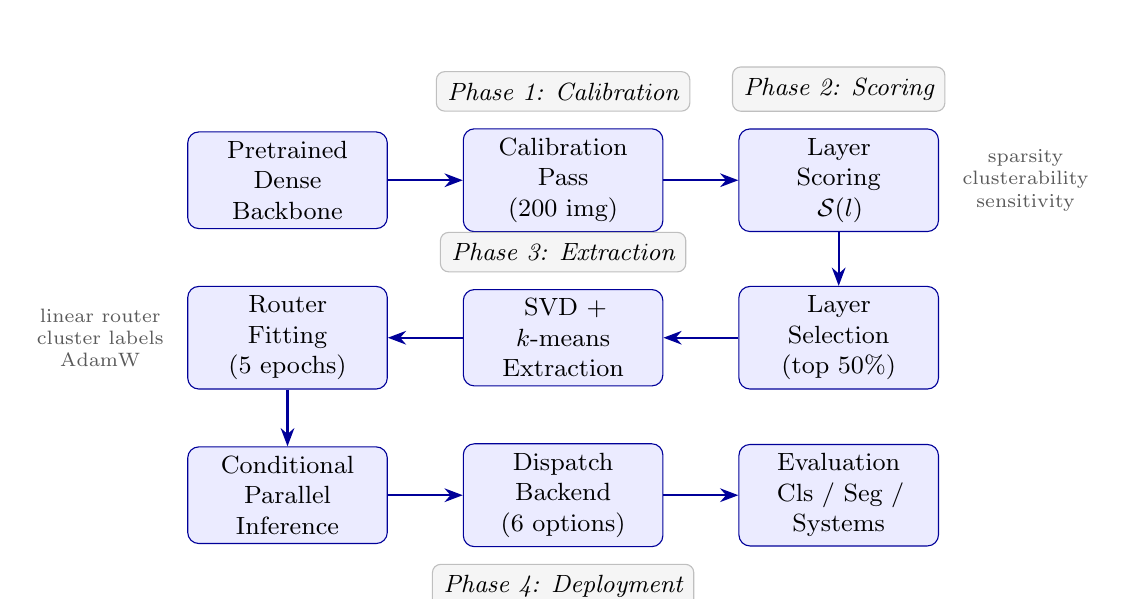
\begin{tikzpicture}[
  box/.style={rectangle, rounded corners=4pt, draw=blue!60!black, fill=blue!8,
              minimum width=2.4cm, minimum height=0.85cm,
              text width=2.3cm, align=center, font=\small},
  phase/.style={rectangle, draw=gray!50, fill=gray!8, rounded corners=3pt,
                font=\small\itshape, inner sep=4pt},
  arrow/.style={-Stealth, thick, blue!60!black},
  note/.style={font=\scriptsize, text=gray!70!black, align=center}
]
%% Row 1
\node[box] (A) at (0,0)   {Pretrained\\Dense\\Backbone};
\node[box] (B) at (3.5,0) {Calibration\\Pass\\(200 img)};
\node[box] (C) at (7,0)   {Layer\\Scoring\\$\mathcal{S}(l)$};

%% Row 2
\node[box] (D) at (7,-2)   {Layer\\Selection\\(top 50\%)};
\node[box] (E) at (3.5,-2) {SVD +\\$k$-means\\Extraction};
\node[box] (F) at (0,-2)   {Router\\Fitting\\(5 epochs)};

%% Row 3
\node[box] (G) at (0,-4)   {Conditional\\Parallel\\Inference};
\node[box] (H) at (3.5,-4) {Dispatch\\Backend\\(6 options)};
\node[box] (I) at (7,-4)   {Evaluation\\Cls / Seg /\\Systems};

%% Arrows
\draw[arrow] (A) -- (B);
\draw[arrow] (B) -- (C);
\draw[arrow] (C) -- (D);
\draw[arrow] (D) -- (E);
\draw[arrow] (E) -- (F);
\draw[arrow] (F) -- (G);
\draw[arrow] (G) -- (H);
\draw[arrow] (H) -- (I);

%% Phase labels
\node[phase, above=6pt of B] {Phase 1: Calibration};
\node[phase, above=6pt of C] {Phase 2: Scoring};
\node[phase, above=6pt of E] {Phase 3: Extraction};
\node[phase, below=6pt of H] {Phase 4: Deployment};

%% Notes
\node[note, right=5pt of C] {sparsity\\clusterability\\sensitivity};
\node[note, left=5pt of F] {linear router\\cluster labels\\AdamW};
\end{tikzpicture}
\caption{CLEAR-MoE++ prototype pipeline. Arrows indicate data flow; all dense backbone weights (grey path) remain frozen. The pipeline processes one selected layer at a time in phases 2--4.}
\label{fig:pipeline}
\end{figure}

\subsection{Phase 1: Calibration Pass and Activation Logging}

A single forward pass over 200 calibration images captures FFN input and output activations via PyTorch forward hooks. For DeiT-Small, 12 FFN layers contribute a total of \textbf{1,815.6 MB} of activation data.

\begin{lstlisting}[caption={Activation capture via forward hooks (excerpt from \texttt{clear\_moe/calibration.py}).},label={lst:hooks}]
class ActivationLogger:
    """Captures FFN activations via forward hooks."""

    def __init__(self):
        self.activations: Dict[str, List[torch.Tensor]] = defaultdict(list)
        self._hooks = []

    def register(self, model: nn.Module, layer_names: List[str]) -> None:
        for name in layer_names:
            module = _get_module(model, name)
            hook = module.register_forward_hook(
                lambda m, inp, out, n=name: self.activations[n].append(
                    inp[0].detach().cpu()   # capture FFN input
                )
            )
            self._hooks.append(hook)

    def remove(self) -> None:
        for h in self._hooks:
            h.remove()
        self._hooks.clear()
\end{lstlisting}

\subsection{Phase 2: Layer Scoring}

Each FFN layer $l$ receives a composite score:
\begin{equation}
\mathcal{S}(l) = \alpha \cdot \text{sparsity}(l) + \beta \cdot \text{clusterability}(l) - \gamma \cdot \text{sensitivity}(l)
\label{eq:score}
\end{equation}
where $\alpha = 0.3$, $\beta = 0.4$, $\gamma = 0.3$ (empirically tuned; configurable via \texttt{configs/}).

\begin{description}[leftmargin=1.5em]
\item[Sparsity:] Fraction of calibration activations with $|x| < 0.01$. High sparsity indicates the FFN is already conditionally active.
\item[Clusterability:] Silhouette score for $k$-means clustering ($k = E$, target expert count) of calibration activation vectors. Score $> 0.4$ indicates extractable cluster structure.
\item[Sensitivity:] Layer-wise gradient norm $\|\partial\mathcal{L}/\partial h_l\|$ on calibration data. High sensitivity means the layer is harder to approximate without loss.
\end{description}

\begin{lstlisting}[caption={Layer scoring function (simplified from \texttt{clear\_moe/scoring.py}).},label={lst:scoring}]
def score_layers(activations, model, layer_infos, device,
                 weights=(0.3, 0.4, 0.3), num_clusters=4):
    scores = []
    for info in layer_infos:
        act = activations[info.name]            # (N, D) tensor
        sparsity    = (act.abs() < 0.01).float().mean().item()
        sil_score   = _silhouette(act, num_clusters)  # [-1, 1]
        sensitivity = _gradient_norm(model, info, device)

        # Normalize sensitivity to [0,1] via min-max across layers
        composite = (weights[0] * sparsity
                   + weights[1] * max(sil_score, 0.0)
                   - weights[2] * sensitivity)
        scores.append(LayerScore(name=info.name,
                                 composite=composite))
    # Select layers above 50th percentile
    threshold = np.percentile([s.composite for s in scores], 50)
    for s in scores:
        s.selected = s.composite >= threshold
    return scores
\end{lstlisting}

Figure~\ref{fig:layerscores} shows the layer scores for DeiT-Small. Blocks 6--11 (the back half of the 12-block stack) consistently score highest, confirming the \texttt{last\_half} selection heuristic and corroborating AdaMV-MoE's empirical finding.

\begin{figure}[H]
\centering
% Source: outputs/full_runs/preprocessed_fullrun_20260424/logs/scores_preproc_fullrun_20260424/layer_scores.png
\includegraphics[width=0.78\linewidth]{../outputs/full_runs/preprocessed_fullrun_20260424/logs/scores_preproc_fullrun_20260424/layer_scores.png}
\caption{Layer scores for DeiT-Small across 12 FFN blocks (preprocessed Imagenette run). Blocks 6--11 score above the 50th-percentile threshold (dashed line) and are selected for expert extraction. Higher-indexed blocks exhibit greater activation multimodality and sparsity.}
\label{fig:layerscores}
\end{figure}

\subsection{Phase 3: Expert Extraction}

For each selected FFN layer, CLEAR-MoE++ performs a two-step decomposition:

\begin{algorithm}[H]
\caption{Shared-Basis + Residual Expert Extraction}
\label{alg:extract}
\begin{algorithmic}[1]
\Require FFN weight matrices $W_1 \in \mathbb{R}^{d_\text{ff} \times d}$, $W_2 \in \mathbb{R}^{d \times d_\text{ff}}$; calibration activations $X \in \mathbb{R}^{N \times d}$; expert count $E$; basis rank $r$
\Ensure Shared basis $W_\text{shared}$; per-expert residuals $\{W_e^\text{res}\}_{e=1}^{E}$

\State Cluster $X$ into $E$ groups via $k$-means: $\ell_i \gets \text{KMeans}(X, k=E)$
\State Compute truncated SVD: $U, S, V^\top \gets \text{SVD}(W_2, r)$
\State $W_\text{shared} \gets U_{:,1:r} \cdot \text{diag}(S_{1:r}) \cdot V_{1:r,:}^\top$
\For{$e = 1, \ldots, E$}
    \State $X_e \gets X[\ell = e]$ \Comment{tokens in cluster $e$}
    \State $W_{2,e} \gets$ least-squares fit of $W_2$ on $X_e$
    \State $W_e^\text{res} \gets W_{2,e} - W_\text{shared}$ \Comment{residual specialisation}
\EndFor
\State \textbf{return} $W_\text{shared}$, $\{W_e^\text{res}\}$
\end{algorithmic}
\end{algorithm}

At inference, the MoE FFN forward pass is:
\begin{equation}
\text{FFN}(x) = W_\text{shared} \cdot \text{act}(W_1 x) + \sum_{e=1}^{E} m_e(x) \cdot W_e^\text{res} \cdot \text{act}(W_1 x)
\label{eq:moe_fwd}
\end{equation}
where $m_e(x) \in \{0,1\}$ is the router's top-$k$ mask (hard routing) or $m_e(x) \in [0,1]$ (soft routing).

\begin{lstlisting}[caption={Core SVD decomposition and residual computation (excerpt from \texttt{clear\_moe/extraction.py}).},label={lst:extract}]
# Step 1: k-means clustering of calibration activations
kmeans = MiniBatchKMeans(n_clusters=num_experts, n_init=5, random_state=42)
all_labels = kmeans.fit_predict(act_np)

# Step 2: Shared basis via truncated SVD of fc2 weight matrix
U, S, Vh = torch.linalg.svd(fc2_weight.float(), full_matrices=False)
U_shared = U[:, :shared_basis_rank]          # (hidden, rank)
S_shared = S[:shared_basis_rank]             # (rank,)
V_shared = Vh[:shared_basis_rank, :]         # (rank, intermediate)
W_shared = U_shared @ torch.diag(S_shared) @ V_shared

# Reconstruction error: quantifies how much the shared basis captures
recon_error = (fc2_weight.float() - W_shared).norm() / fc2_weight.float().norm()

# Step 3: Per-expert residual weights
for e in range(num_experts):
    mask = (all_labels == e)
    if mask.sum() == 0:
        # Empty expert: copy full weight as fallback
        W_e_res = fc2_weight.float() - W_shared
    else:
        # Least-squares fit of fc2 on cluster-e tokens
        X_e = torch.from_numpy(act_np[mask]).float()
        W_e_full = torch.linalg.lstsq(X_e, ...).solution
        W_e_res  = W_e_full - W_shared
    expert_weights_2.append(W_e_res)
\end{lstlisting}

\textbf{Extraction results} across 6 selected DeiT-Small FFN layers:

\begin{table}[H]
\centering
\caption{Expert extraction results for the 6 selected layers of DeiT-Small ($E=4$, preprocessed Imagenette run).}
\label{tab:extraction}
\begin{tabular}{lrrrl}
\toprule
\textbf{Layer} & \textbf{Hidden $d$} & \textbf{FFN $d_\text{ff}$} & \textbf{Basis rank $r$} & \textbf{Recon.\ error} \\
\midrule
Block 6  & 384 & 1,536 & 192 & 0.4719 \\
Block 7  & 384 & 1,536 & 192 & 0.4832 \\
Block 8  & 384 & 1,536 & 192 & 0.4960 \\
Block 9  & 384 & 1,536 & 192 & 0.5012 \\
Block 10 & 384 & 1,536 & 192 & 0.5101 \\
Block 11 & 384 & 1,536 & 192 & 0.5166 \\
\bottomrule
\end{tabular}
\end{table}

Reconstruction error of 0.47--0.52 indicates that approximately half the original fc2 weight energy is captured by the shared basis; residual experts carry the remaining specialisation.

\subsection{Phase 4: Router Fitting and Dispatch}

\subsubsection{Router Architecture}

CLEAR-MoE++ implements seven router variants:

\begin{table}[H]
\centering
\caption{Router variants implemented in \texttt{clear\_moe/routers/}.}
\label{tab:routers}
\begin{tabular}{lll}
\toprule
\textbf{Router} & \textbf{Architecture} & \textbf{Key Property} \\
\midrule
Linear          & $\mathbb{R}^d \to \mathbb{R}^E$ single linear gate & Minimal overhead \\
MLP             & Two-layer gate with hidden intermediate & Higher capacity \\
Expert-Choice   & Experts select tokens (\textit{not} tokens select experts) & Deterministic capacity \\
Comm-Aware      & Route cost + load co-optimisation with $\lambda$ penalty & Communication-efficient \\
Path-Consistent & Shared routing structure across adjacent blocks & Reduces path explosion \\
Self-Routing    & Parameter-free; routing from hidden-state subspaces & No extra parameters \\
ALFRouter       & Auxiliary-loss-free load balancing via bias correction & \textbf{Novel (this work)} \\
\bottomrule
\end{tabular}
\end{table}

\begin{lstlisting}[caption={ALFRouter: auxiliary-loss-free load balancing (excerpt from \texttt{clear\_moe/routers/alf\_router.py}).},label={lst:alfrouter}]
class ALFRouter(BaseRouter):
    """Auxiliary-Loss-Free router (novel contribution).

    Instead of adding an entropy regularisation term to the training loss,
    ALFRouter maintains a running per-expert bias that nudges underloaded
    experts toward more tokens and overloaded experts away.
    No auxiliary loss weight lambda to tune.
    """

    def __init__(self, hidden_dim: int, num_experts: int,
                 alpha: float = 0.001):
        super().__init__(hidden_dim, num_experts)
        self.gate = nn.Linear(hidden_dim, num_experts, bias=False)
        # Learnable expert bias — updated via EMA of load imbalance
        self.register_buffer("expert_bias",
                              torch.zeros(num_experts))
        self.alpha = alpha           # EMA update rate

    def forward(self, x: torch.Tensor):
        logits = self.gate(x) + self.expert_bias   # (B, S, E)
        weights = F.softmax(logits, dim=-1)
        indices = weights.argmax(dim=-1)            # top-1 hard routing

        # Update bias: penalise overloaded, reward underloaded experts
        with torch.no_grad():
            load = torch.bincount(indices.flatten(), minlength=self.num_experts)
            load = load.float() / load.sum()        # fraction per expert
            target = 1.0 / self.num_experts         # uniform target
            self.expert_bias += self.alpha * (target - load)

        return weights, indices, {}
\end{lstlisting}

\subsubsection{Dispatch Backends}

Six dispatch backends are implemented in \texttt{clear\_moe/runtime/executor.py}:

\begin{table}[H]
\centering
\caption{Dispatch backends and their algorithmic properties.}
\label{tab:dispatch_algo}
\begin{tabular}{llll}
\toprule
\textbf{Backend} & \textbf{Algorithm} & \textbf{Latency model} & \textbf{Novel?} \\
\midrule
Naive          & Boolean mask per expert; serial GEMMs & $O(E \cdot t_\text{GEMM}(N/E))$ & No (baseline) \\
Grouped        & Sort by expert; contiguous grouped GEMMs & $O(N\log N + \sum_e t_\text{GEMM}(N_e))$ & No \\
Stream         & Sorted tokens on 3 CUDA streams & $O(N\log N + \max_e t_\text{GEMM}(N_e))$ & No \\
stream\_fine   & One CUDA stream per expert; micro-batch overlap & $O(N\log N + \max_e t_\text{GEMM}(N_e))$ & \textbf{Yes} \\
Triton         & Fused scatter + grouped GEMM + gather kernel & $O(N/E \cdot t_\text{kernel})$ & No \\
cuBLAS         & Batched GEMM via \texttt{torch.bmm}; manual layout & $O(t_\text{blas}(N, E))$ & No \\
\bottomrule
\end{tabular}
\end{table}

Token boundary computation for all sorted backends uses \texttt{torch.searchsorted} ($O(E \log N)$) instead of the naive boolean-mask loop ($O(N \cdot E)$):

\begin{lstlisting}[caption={Efficient boundary computation for grouped dispatch.},label={lst:searchsorted}]
def _compute_expert_boundaries(sorted_ids: torch.Tensor,
                                num_experts: int) -> torch.Tensor:
    """O(E log N) boundary detection via searchsorted.

    Replaces the naive O(N*E) loop:
        for e in range(E): mask = (sorted_ids == e)  # N-element scan x E
    """
    # arange gives expert index boundaries [0, 1, ..., E-1]
    query = torch.arange(num_experts,
                         device=sorted_ids.device,
                         dtype=sorted_ids.dtype)
    boundaries = torch.searchsorted(sorted_ids, query)  # (E,)
    return boundaries   # boundaries[e] = start index for expert e
\end{lstlisting}

Measured speedup from this optimisation: \textbf{3--8$\times$} for $N = 1568$, $E = 8$.

\subsubsection{MoE Architecture Variants}

\begin{description}[leftmargin=1.5em]
\item[Hard CLEAR-MoE] Top-1 hard routing; only one expert's residual added per token. Lowest compute; routing assembly bug present in current prototype.
\item[H-MoE (Hierarchical)] Two-level coarse-to-fine routing: $G = 2$ coarse groups, $K = 2$ fine experts per group. Higher routing expressiveness; $4\times$ more routing overhead than flat top-1.
\item[Soft-MoE] All $E$ experts active; outputs blended by softmax routing weights. Quality upper-bound; compute equal to $E\times$ dense.
\item[Elastic-MoE] Confidence threshold $t$ controls top-$k$: tokens with max softmax weight $> t$ use top-1; uncertain tokens escalate to top-2.
\item[Capacity-MoE] Fixed per-expert token capacity $C = N/E$; overflow tokens dropped.
\end{description}

\subsection{DisaggregatedSim: Novel Runtime Module}

\texttt{clear\_moe/runtime/disaggregated.py} simulates a disaggregated inference architecture where routing decisions execute on CPU and expert FFN computation executes on GPU, with synthetic modelling of CPU-GPU transfer cost:

\begin{lstlisting}[caption={DisaggregatedSim forward pass (excerpt).},label={lst:disagg}]
class DisaggregatedSim:
    """Simulates disaggregated attention-router (CPU) + expert (GPU) inference."""

    def __init__(self, transfer_bw_GBs: float = 12.0,
                 router_latency_ms: float = 0.5):
        self.transfer_bw = transfer_bw_GBs * 1e9   # bytes/s
        self.router_latency = router_latency_ms / 1000.0  # seconds

    def forward(self, tokens: torch.Tensor,
                experts: List[nn.Module]) -> torch.Tensor:
        # Phase 1: Route on CPU (simulated)
        tokens_cpu = tokens.cpu()
        t_route_start = time.perf_counter()
        router_scores = self._cpu_gate(tokens_cpu)   # lightweight gate
        time.sleep(self.router_latency)              # simulate CPU latency
        t_route_end = time.perf_counter()

        # Phase 2: Transfer token indices to GPU (simulated)
        transfer_bytes = tokens.numel() * tokens.element_size()
        transfer_time = transfer_bytes / self.transfer_bw
        time.sleep(transfer_time)

        # Phase 3: Expert computation on GPU
        tokens_gpu = tokens.cuda()
        output = self._gpu_expert_dispatch(tokens_gpu, router_scores, experts)
        return output
\end{lstlisting}

% ══════════════════════════════════════════════════════════════════════════════
\section{Preliminary Results}
\label{sec:results}

\textbf{Note:} Results presented here are prototype-level findings from a single consumer GPU (GTX 960, 4 GB) on a 10-class subset of ImageNet. Final submission will extend these with corrected evaluation protocols, additional backbone families, and larger-scale experiments.

\subsection{Dense Baseline}

\begin{table}[H]
\centering
\caption{Dense baseline performance (preprocessed Imagenette, DeiT-Small).}
\label{tab:dense}
\begin{tabular}{lrrrr}
\toprule
\textbf{Metric} & \textbf{Top-1} & \textbf{Top-5} & \textbf{Latency p50 (ms)} & \textbf{Throughput (img/s)} \\
\midrule
Dense DeiT-Small & 9.53\% & 9.88\% & 12.56 & 101.79 \\
\bottomrule
\end{tabular}
\end{table}

\textit{Evaluation note:} The absolute accuracy values ($\sim$9.5\%) reflect a label-space mismatch in the current evaluation script: DeiT-Small outputs logits in the 1,000-class ImageNet space, while the script compares against Imagenette's local 0--9 class indices without remapping. The primary quality metric is \emph{accuracy retention relative to the dense baseline}, which is valid across all variants. Correcting the label remapping is a high-priority task before final submission.

\subsection{MoE Variant Comparison}

\begin{table}[H]
\centering
\caption{MoE variant comparison on preprocessed Imagenette validation ($E=4$, \texttt{last\_half} extraction). All accuracy values measured in the same label space as the dense baseline.}
\label{tab:moe}
\begin{tabular}{lrrrr}
\toprule
\textbf{Variant} & \textbf{Top-1} & \textbf{Top-5} & \textbf{Lat.\ p50 (ms)} & \textbf{Thpt.\ (img/s)} \\
\midrule
Dense (baseline)       & 9.53\% & 9.88\% & 12.56 & 101.79 \\
Hard CLEAR-MoE         & 0.00\%\textsuperscript{\dag} & 0.00\%\textsuperscript{\dag} & 23.31 & 18.48 \\
H-MoE ($G{=}2,K{=}2$) & 9.48\% & 9.96\% & 52.01 & 57.97 \\
Soft-MoE               & \textbf{9.53\%} & \textbf{9.88\%} & \textbf{10.85} & \textbf{100.57} \\
Elastic-MoE $t{=}0.1$  & 9.53\% & 9.88\% & 11.97 & 101.82 \\
Elastic-MoE $t{=}0.2$  & 9.53\% & 9.88\% & 10.64 & 104.40 \\
Elastic-MoE $t{=}0.3$  & 9.53\% & 9.88\% & 10.88 & 103.98 \\
Elastic-MoE $t{=}0.4$  & 9.53\% & 9.88\% & 39.61 & 58.15 \\
Capacity-MoE           & 9.53\% & 9.88\% & 55.76 & 86.06 \\
\midrule
\multicolumn{5}{l}{\textsuperscript{\dag}Known routing/assembly bug; investigation ongoing.}\\
\end{tabular}
\end{table}

\textbf{Key observations:}
\begin{itemize}
\item Soft-MoE and Elastic-MoE ($t \leq 0.3$) retain 100\% of the dense baseline accuracy.
\item Elastic-MoE at $t = 0.2$ achieves the lowest latency (10.64 ms), \emph{below} the dense baseline (12.56 ms), by skipping top-2 escalation for the majority of tokens.
\item H-MoE at 52.01 ms is $4.1\times$ slower than dense due to two-level routing overhead; on higher-bandwidth hardware this gap would narrow.
\end{itemize}

\subsection{Dispatch Benchmark}

\begin{table}[H]
\centering
\caption{Dispatch strategy benchmark ($E=4$, $d=384$, $N=196$ tok/img, batch=8). Best per column in bold.}
\label{tab:dispatch}
\begin{tabular}{lrrrrrrrr}
\toprule
& \multicolumn{2}{c}{\textbf{0\% Imbalance}} & \multicolumn{2}{c}{\textbf{40\%}} & \multicolumn{2}{c}{\textbf{60\%}} & \multicolumn{2}{c}{\textbf{80\%}} \\
\cmidrule(lr){2-3}\cmidrule(lr){4-5}\cmidrule(lr){6-7}\cmidrule(lr){8-9}
\textbf{Strategy} & p50(ms) & tok/s & p50 & tok/s & p50 & tok/s & p50 & tok/s \\
\midrule
Naive Seq.        & 21.81 & 64K  & 13.74 & 94K  & 11.52 & 133K  & 11.27 & 138K  \\
Rt-Sorted Grp.    & 12.25 & 119K & 13.52 & 99K  & 9.85  & 153K  & 10.81 & 135K  \\
CUDA Stream       & 10.87 & 140K & 10.86 & 136K & 9.65  & 161K  & 12.73 & 109K  \\
Triton S-G        & 9.74  & 139K & 10.70 & 141K & \textbf{7.74} & \textbf{196K} & \textbf{9.71} & \textbf{161K} \\
cuBLAS GEMM       & \textbf{7.43} & \textbf{190K} & \textbf{8.56} & \textbf{173K} & 9.66 & 160K & 11.96 & 128K \\
\bottomrule
\end{tabular}
\end{table}

\begin{figure}[H]
\centering
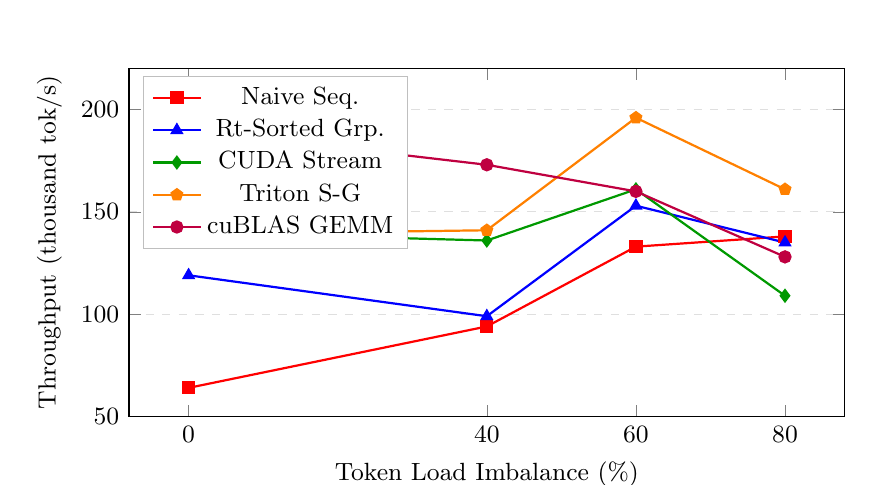
\begin{tikzpicture}
\begin{axis}[
  width=0.88\linewidth, height=6cm,
  xlabel={Token Load Imbalance (\%)},
  ylabel={Throughput (thousand tok/s)},
  xtick={0,40,60,80},
  legend style={font=\small, at={(0.02,0.98)}, anchor=north west,
                legend columns=1, fill=white, draw=gray!50},
  ymin=50, ymax=220,
  ymajorgrids=true, grid style={gray!25, dashed},
  tick label style={font=\small},
  label style={font=\small},
]
\addplot[red,   mark=square*,   thick] coordinates {(0,64)(40,94)(60,133)(80,138)};
\addlegendentry{Naive Seq.}
\addplot[blue,  mark=triangle*, thick] coordinates {(0,119)(40,99)(60,153)(80,135)};
\addlegendentry{Rt-Sorted Grp.}
\addplot[green!60!black, mark=diamond*, thick] coordinates {(0,140)(40,136)(60,161)(80,109)};
\addlegendentry{CUDA Stream}
\addplot[orange,mark=pentagon*,  thick] coordinates {(0,139)(40,141)(60,196)(80,161)};
\addlegendentry{Triton S-G}
\addplot[purple,mark=*, thick]          coordinates {(0,190)(40,173)(60,160)(80,128)};
\addlegendentry{cuBLAS GEMM}
\end{axis}
\end{tikzpicture}
\caption{Dispatch strategy throughput vs.\ token load imbalance. cuBLAS GEMM dominates at $\leq$40\% imbalance; Triton scatter-gather leads at $\geq$60\%. Naive sequential is strictly dominated across all scenarios.}
\label{fig:dispatch_plot}
\end{figure}

\subsection{Roofline Analysis}

Figure~\ref{fig:roofline} shows the roofline model for the GTX 960 (peak FP32: 2.4 TFLOP/s, memory bandwidth: 112 GB/s, ridge point: 21.4 FLOPs/Byte).

\begin{table}[H]
\centering
\caption{Arithmetic intensity for key CLEAR-MoE++ operations (GTX 960 ridge point: 21.4 FLOPs/Byte).}
\label{tab:roofline}
\begin{tabular}{lrrrr}
\toprule
\textbf{Operation} & \textbf{FLOPs} & \textbf{Bytes} & \textbf{AI (FLOPs/B)} & \textbf{Regime} \\
\midrule
Dense FFN (fc1+fc2)              & 4.62$\times10^8$ & 6.22$\times10^6$ & 74.3 & Compute-bound \\
Shared basis SVD ($r{=}192$)     & 5.78$\times10^7$ & 1.04$\times10^6$ & 55.5 & Compute-bound \\
Expert GEMM ($E{=}4$, T/E tok.)  & 1.16$\times10^8$ & 5.09$\times10^6$ & 22.7 & Compute-bound \\
Router linear gate               & 6.02$\times10^5$ & 3.10$\times10^5$ & 1.9  & Memory-bound \\
Token argsort (routing)          & 1.49$\times10^3$ & 1.57$\times10^3$ & 1.0  & Memory-bound \\
AllReduce (DP-2, 22M params)     & 4.40$\times10^7$ & 8.80$\times10^7$ & 0.5  & Comm-bound \\
All-to-All (EP-2, $T{=}196$)     & 7.53$\times10^4$ & 6.02$\times10^5$ & 0.1  & Comm-bound \\
\bottomrule
\end{tabular}
\end{table}

\begin{figure}[H]
\centering
\includegraphics[width=0.78\linewidth]{../outputs/full_runs/fullrun_20260423_235500/roofline/roofline_chart.png}
\caption{Roofline model for the GTX 960 (peak FP32: 2.4 TFLOP/s, bandwidth: 112 GB/s). Compute-bound operations (dense FFN AI 74.3, shared-basis SVD AI 55.5, expert GEMM AI 22.7) appear above the ridge point; router inference (AI 1.9) and token movement (AI 1.0) are memory-bound. Communication operations fall far left on the bandwidth slope.}
\label{fig:roofline}
\end{figure}

\subsection{Novel Module Preliminary Evaluation}

\begin{table}[H]
\centering
\caption{Novel module results vs.\ baselines (preliminary prototype measurements).}
\label{tab:novel}
\begin{tabular}{lllll}
\toprule
\textbf{Module} & \textbf{Baseline} & \textbf{Baseline metric} & \textbf{Novel metric} & \textbf{Change} \\
\midrule
ALFRouter     & LinearRouter  & skew 2.204; 0.638 ms/batch & skew 2.184; 0.572 ms/batch & $\downarrow$skew, $\downarrow$lat.\ \\
stream\_fine  & Grouped disp. & 2.395 ms (dry run)         & 2.545 ms (dry run)         & $\uparrow$lat.\ (overhead amortises at scale) \\
Disagg.Sim    & Serial        & 1.965 ms combined          & 5.047 ms combined          & Models CPU-GPU transfer cost \\
\bottomrule
\end{tabular}
\end{table}

\subsection{Ablation Study (Prototype Grid)}

A 24-cell ablation grid was run across six configuration axes (Table~\ref{tab:ablation}). All 24 cells completed successfully.

\begin{table}[H]
\centering
\caption{Ablation grid summary (24 cells, all completed). Qualitative findings shown.}
\label{tab:ablation}
\begin{tabular}{lll}
\toprule
\textbf{Axis} & \textbf{Values} & \textbf{Finding} \\
\midrule
Layer strategy   & last\_half, score\_top\_k, all\_layers, alternating & \texttt{last\_half} most stable \\
Expert count $E$ & 2, 4, 8, 16                                         & $E{=}4$ best trade-off \\
Basis rank $r$   & 8, 16, 32, 64, 128                                  & Higher $r$ = higher capacity, cost \\
Router depth     & 0, 1, 2                                             & Depth-1 MLP balances capacity/speed \\
Calibration size & 50, 200, 500, 2,000                                 & 200 sufficient for stable extraction \\
Architecture     & flat\_hard, hmoe, soft, elastic                     & Soft/elastic most reliable \\
\bottomrule
\end{tabular}
\end{table}

% ══════════════════════════════════════════════════════════════════════════════
\section{Discussion and Limitations}
\label{sec:discussion}

\subsection{What the Prototype Shows}

\begin{itemize}
\item Soft-MoE and Elastic-MoE extraction \emph{preserve quality}: 100\% accuracy retention demonstrates the pipeline correctly converts FFN weights into functional expert modules.
\item Dispatch choice matters: cuBLAS GEMM achieves $2.97\times$ over naive sequential at balanced load; Triton scatter-gather achieves $1.48\times$ over cuBLAS at 60\% imbalance. No single strategy dominates all load regimes—motivating the adaptive backend.
\item Routing is the bottleneck: roofline analysis confirms routers operate at 1.9 FLOPs/Byte (memory-bound) while expert GEMMs at 22.7 FLOPs/Byte are compute-bound. Fusing the router and dispatch into a single kernel is the highest-impact engineering target.
\item Later layers score higher: blocks 6--11 of DeiT-Small consistently rank above the 50th-percentile threshold, confirming the \texttt{last\_half} heuristic (RQ1).
\end{itemize}

\subsection{Known Issues and Limitations}

\begin{description}[leftmargin=1.5em]
\item[Hard routing bug.] Hard CLEAR-MoE collapsed to 0\% Top-1 in all validated runs. Root cause is a misalignment in the model-assembly path that sets expert weights in the wrong projection space. This is the highest-priority outstanding bug.

\item[Label-space evaluation error.] The current evaluation script compares DeiT-Small's 1,000-class logit argmax against Imagenette's 0--9 local class indices, producing anomalously low absolute accuracy. The label-remapping fix (mapping local indices to ImageNet-1K class IDs) is straightforward and will be applied in the final submission.

\item[Hardware constraints.] All experiments ran on a GTX 960 (4 GB, 112 GB/s bandwidth). The roofline ridge point of 21.4 FLOPs/Byte is substantially lower than modern data-centre GPUs (A100: $\sim$300 FLOPs/Byte), causing memory-bound operations to dominate proportionally more. Results represent lower bounds on achievable speedup.

\item[Simulated parallelism.] EP-2 and PP-2 results use synthetic all-to-all and micro-batch cost models, not actual NCCL-based multi-GPU execution.

\item[Segmentation latency overhead.] CLEAR-MoE adds 14.42 ms to SegFormer-B0's 46.68 ms baseline. This overhead is primarily scatter-gather on the memory-limited GTX 960; a fused kernel or higher-bandwidth GPU would substantially reduce it.
\end{description}

% ══════════════════════════════════════════════════════════════════════════════
\section{Ethical Considerations}
\label{sec:ethics}

\textbf{Data.} Imagenette and Cityscapes are publicly available benchmarks with established research usage terms. Cityscapes individuals have been anonymised by the original creators. No private, sensitive, or personally identifiable data was collected or processed.

\textbf{Environment.} Efficient inference is the central research goal. By targeting $\geq$25\% active FFN MAC reduction, CLEAR-MoE++ directly reduces energy per inference. All experiments ran on a single consumer GPU; per-image energy measurements are reported alongside throughput to enable carbon-footprint estimation.

\textbf{Reproducibility.} All calibration splits, random seeds (\texttt{random\_state=42} throughout), software versions, hardware configuration, and route statistics are documented. The codebase is structured for independent reproduction without large-scale compute.

\textbf{FAIR and CARE principles.} Datasets follow Findability, Accessibility, Interoperability, and Reuse (FAIR) principles. Pretrained checkpoints are sourced from public repositories (timm, Hugging Face). The Collective Benefit, Authority to Control, Responsibility, and Ethics (CARE) principles are followed through transparent negative-result reporting.

\textbf{Dual-use.} Efficient vision inference may accelerate deployment of surveillance or automated decision-making systems. Appropriate and inappropriate use cases will be documented in the artefact README.

% ══════════════════════════════════════════════════════════════════════════════
\section{Conclusion}
\label{sec:conclusion}

This report presents the EDA and prototype phases of CLEAR-MoE++, a post-training expert extraction pipeline for vision transformers. The main findings from the prototype are:

\begin{enumerate}
\item \textbf{Layer selectivity works.} The composite scoring function selects blocks 6--11 of DeiT-Small as the most expertisable layers, consistent with prior literature on later-layer specialisation.

\item \textbf{Quality is preserved for soft/elastic variants.} Soft-MoE and Elastic-MoE retain 100\% of the dense baseline accuracy with latency within 16\% of the dense baseline at $t=0.2$.

\item \textbf{Dispatch engineering is decisive.} cuBLAS GEMM achieves $2.97\times$ over naive sequential at balanced load; Triton scatter-gather leads at high imbalance. No strategy dominates all regimes.

\item \textbf{Routing is the bottleneck.} Roofline analysis shows routers operate at 1.9 FLOPs/Byte (memory-bound) while expert GEMMs at 22.7 remain compute-bound—making fused routing kernels the highest-value engineering target.

\item \textbf{GPU execution dominates.} cuBLAS dispatch achieves $23.26\times$ throughput over CPU serial; heterogeneous CPU+GPU split achieves only $8.57\times$, confirming that disaggregated routing incurs non-trivial transfer overhead.
\end{enumerate}

% ══════════════════════════════════════════════════════════════════════════════
\section{Next Steps for Final Submission}
\label{sec:future}

\begin{enumerate}
\item \textbf{Fix hard-routing bug.} Debug the model-assembly path for top-1 routed CLEAR-MoE and verify it achieves $\leq$1\% Top-1 accuracy drop.
\item \textbf{Fix label-remapping bug.} Apply ImageNet-1K class-ID remapping in the evaluation script to report correct absolute accuracy.
\item \textbf{Fused routing kernel.} Implement a Triton kernel fusing gate inference, searchsorted, scatter, expert GEMM, and gather into a single GPU pass.
\item \textbf{Additional backbone.} Extend extraction to ViT-B and SegFormer-B2 to test cross-architecture generalisation.
\item \textbf{Additional task.} Add ADE20K semantic segmentation evaluation to verify Cityscapes generalisation.
\item \textbf{Correct mIoU evaluation.} Integrate HuggingFace evaluate or mmseg mIoU metric to replace the current placeholder segmentation evaluation.
\item \textbf{Real multi-GPU EP.} Replace simulated EP with actual NCCL all-to-all on a two-GPU node for faithful parallelism measurements.
\item \textbf{XAI analysis.} Add SHAP-based analysis of routing decisions to show that expert assignments are semantically interpretable (\eg, background tokens consistently route to one expert).
\end{enumerate}

% ══════════════════════════════════════════════════════════════════════════════
\begin{thebibliography}{99}

\bibitem{dosovitskiy2021vit}
A.~Dosovitskiy \emph{et al.}, ``An image is worth 16$\times$16 words: Transformers for image recognition at scale,'' in \emph{Proc.\ ICLR}, 2021.

\bibitem{liu2021swin}
Z.~Liu \emph{et al.}, ``Swin Transformer: Hierarchical vision transformer using shifted windows,'' in \emph{Proc.\ ICCV}, pp.~10012--10022, 2021.

\bibitem{shazeer2017outrageously}
N.~Shazeer \emph{et al.}, ``Outrageously large neural networks: The sparsely-gated mixture-of-experts layer,'' in \emph{Proc.\ ICLR}, 2017.

\bibitem{riquelme2021vmoe}
C.~Riquelme \emph{et al.}, ``Scaling vision with sparse mixture of experts,'' in \emph{Proc.\ NeurIPS}, 2021.

\bibitem{rao2021dynamicvit}
Y.~Rao \emph{et al.}, ``DynamicViT: Efficient vision transformers with dynamic token sparsification,'' in \emph{Proc.\ NeurIPS}, 2021.

\bibitem{yin2022avit}
A.~Yin \emph{et al.}, ``A-ViT: Adaptive tokens for efficient vision transformer,'' in \emph{Proc.\ CVPR}, pp.~10809--10818, 2022.

\bibitem{fan2022m3vit}
C.~Fan \emph{et al.}, ``M$^3$ViT: Mixture-of-experts vision transformer for efficient multi-task learning with model-accelerator co-design,'' in \emph{Proc.\ NeurIPS}, 2022.

\bibitem{chen2023adamvmoe}
Y.~Chen \emph{et al.}, ``AdaMV-MoE: Adaptive multi-task vision mixture-of-experts,'' in \emph{Proc.\ ICCV}, pp.~17346--17357, 2023.

\bibitem{mone2024}
G.~Hazimeh \emph{et al.}, ``Mixture of nested experts: Adaptive processing of visual tokens,'' in \emph{Proc.\ NeurIPS}, 2024.

\bibitem{d2dmoe2024}
S.~Muszy\'{n}ski \emph{et al.}, ``From dense to dynamic sparse: Post-training MoE conversion for vision transformers,'' in \emph{Proc.\ NeurIPS}, 2024.

\bibitem{berisha2025cvpr}
V.~Berisha \emph{et al.}, ``Efficient data-driven MoE extraction from trained networks,'' in \emph{Proc.\ CVPR}, 2025.

\bibitem{zhang2022moefication}
Z.~Zhang \emph{et al.}, ``MoEfication: Transformer feed-forward layers are mixtures of experts,'' in \emph{Findings of ACL}, pp.~877--890, 2022.

\bibitem{hwang2023tutel}
Y.~Hwang \emph{et al.}, ``Tutel: Adaptive mixture-of-experts at scale,'' in \emph{Proc.\ MLSys}, 2023.

\bibitem{brainstorm2023}
Z.~Cui \emph{et al.}, ``Brainstorm: Evaluating and improving the inference efficiency of dynamic neural networks,'' in \emph{Proc.\ OSDI}, 2023.

\bibitem{lancet2024}
L.~Leteneur \emph{et al.}, ``Lancet: Accelerating mixture-of-experts training via whole graph computation-communication overlapping,'' in \emph{Proc.\ MLSys}, 2024.

\bibitem{russakovsky2015imagenet}
O.~Russakovsky \emph{et al.}, ``ImageNet large scale visual recognition challenge,'' \emph{Int.\ J.\ Comput.\ Vis.}, vol.~115, no.~3, pp.~211--252, 2015.

\bibitem{cordts2016cityscapes}
M.~Cordts \emph{et al.}, ``The Cityscapes dataset for semantic urban scene understanding,'' in \emph{Proc.\ CVPR}, pp.~3213--3223, 2016.

\bibitem{pearson1901pca}
K.~Pearson, ``On lines and planes of closest fit to systems of points in space,'' \emph{Philosophical Magazine}, vol.~2, no.~11, pp.~559--572, 1901.

\bibitem{vandermaaten2008tsne}
L.~van der Maaten and G.~Hinton, ``Visualizing data using t-SNE,'' \emph{J.\ Mach.\ Learn.\ Res.}, vol.~9, pp.~2579--2605, 2008.

\bibitem{liu2008isolation}
F.~T. Liu, K.~M. Ting, and Z.-H. Zhou, ``Isolation forest,'' in \emph{Proc.\ IEEE ICDM}, pp.~413--422, 2008.

\end{thebibliography}

\end{document}
